\documentclass[tikz,border=5mm]{standalone}
\usepackage{tikz}

\begin{document}
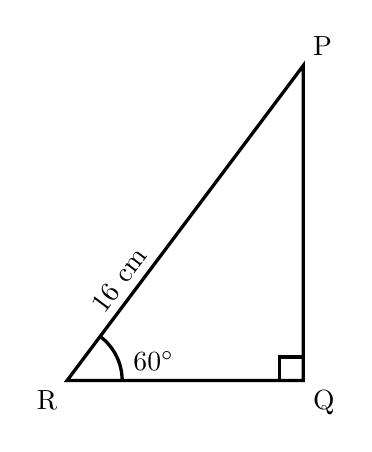
\begin{tikzpicture}

% Define the coordinates
\coordinate (R) at (0,0);
\coordinate (Q) at (3,0);
\coordinate (P) at (3,4);

% Draw the triangle
\draw[very thick] (R) -- (Q) -- (P) -- cycle;

% Draw the right angle mark at Q
\draw[very thick] (Q) ++(-0.3,0) -- ++(0,0.3) -- ++(0.3,0);

% Draw the 60 degree angle arc at R
\draw[very thick] (0.7,0) arc[start angle=0, end angle=53, radius=0.7];
\node at (1.1,0.25) {$60^{\circ}$};

% Label the vertices
\node[below left] at (R) {R};
\node[below right] at (Q) {Q};
\node[above right] at (P) {P};

% Label the side length (16 cm along RP)
\node[above left, rotate=53] at (1.2,1.6) {16 cm};

\end{tikzpicture}
\end{document}